\section{Results}
\label{sec:results}
\begin{table}
	\begin{center}
		\begin{tabular}{|p{0.2\linewidth}|p{0.2\linewidth}|p{0.2\linewidth}|} \hline
			Method & Mean Version & Standard Deviation \\ \hline
			Two Planes & 8.9\degree & 4.7\degree \\
			Corrected Friedman & 8.4\degree & 6.5\degree \\
			Friedman & 9.4\degree & 7.4\degree \\
			Vault & 12.3\degree & 7.7\degree \\
			Commercial software & 9.9\degree & 6.1\degree \\
                        \hline
		\end{tabular}
	\end{center}
	\caption{\label{tab:results}A comparison of the results of each method tested 
	on 10 retrospective patients}
\end{table}

Table \ref{tab:results} presents the results of using \sksglenoid on 10 patients.
The version measured using the planes method has a mean glenoid
version of 8.9\degree (SD, 4.7\degree; range, 5\degree to 20.9\degree), 
while mean glenoid version 
for the 3D corrected Friedman method 
was 8.4\degree (SD, 6.5\degree; range, -4.0\degree to 16.9\degree). 
For the 2D methods, the mean glenoid version for the 
Friedman method was 9.4\degree (SD, 7.4\degree; range, -0.7\degree to 24\degree) 
and for the vault model was 12.3\degree (SD, 7.7\degree; range, 4\degree to 26\degree).
In this 
case a positive value indicates retroversion while a negative value indicates anteversion of the 
glenoid. Overall, the 3D methods resulted in both lower mean version values as well as lower
variability, while the 2D methods revealed a slightly higher variability.

The measurements using these methods were also compared with version measurements on the same
10 patients using a commercial software\cite{djosurgical}. 
The planes method (r = 0.90, p = 0.0004), 
corrected Friedman method (r = 0.83, p = 0.0034), 
and conventional Friedman method (r = 0.79, p = 0.0064) 
all showed significant correlation with the commercial software. 
The vault method did not show significant correlation (r = 0.59, p = 0.074).  
The mean difference between the methods were overall not significant (p > 0.05), 
except for the vault method (p = 0.03). Correlation plots are shown in Figure \ref{fig:correl}.

\begin{figure}
	\begin{center}
		\begin{subfigure}[b]{0.30\linewidth}
			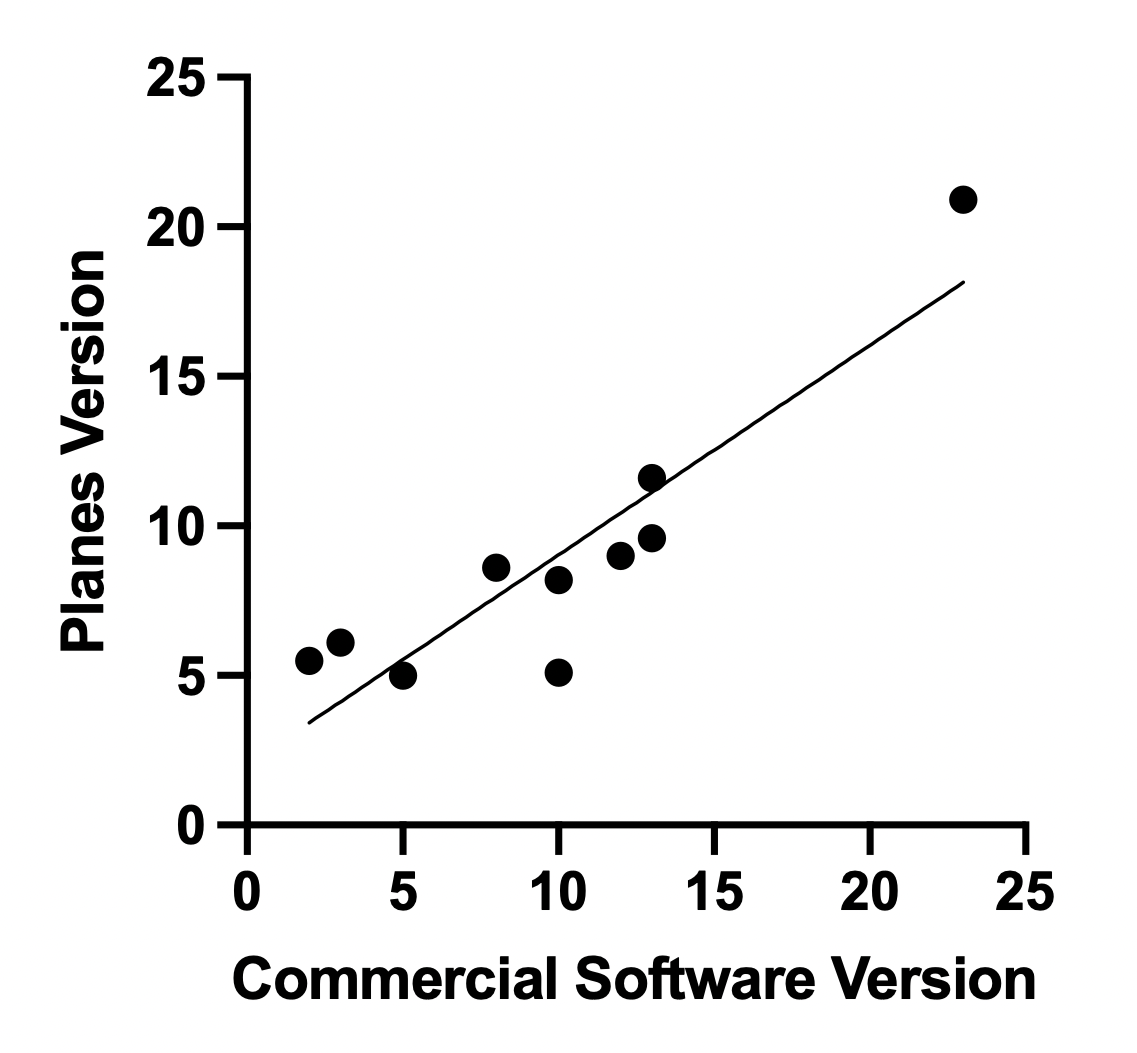
\includegraphics[width=\linewidth]{figures/planes.png}
			\caption{Two Planes Method}
		\end{subfigure}
		\begin{subfigure}[b]{0.30\linewidth}
			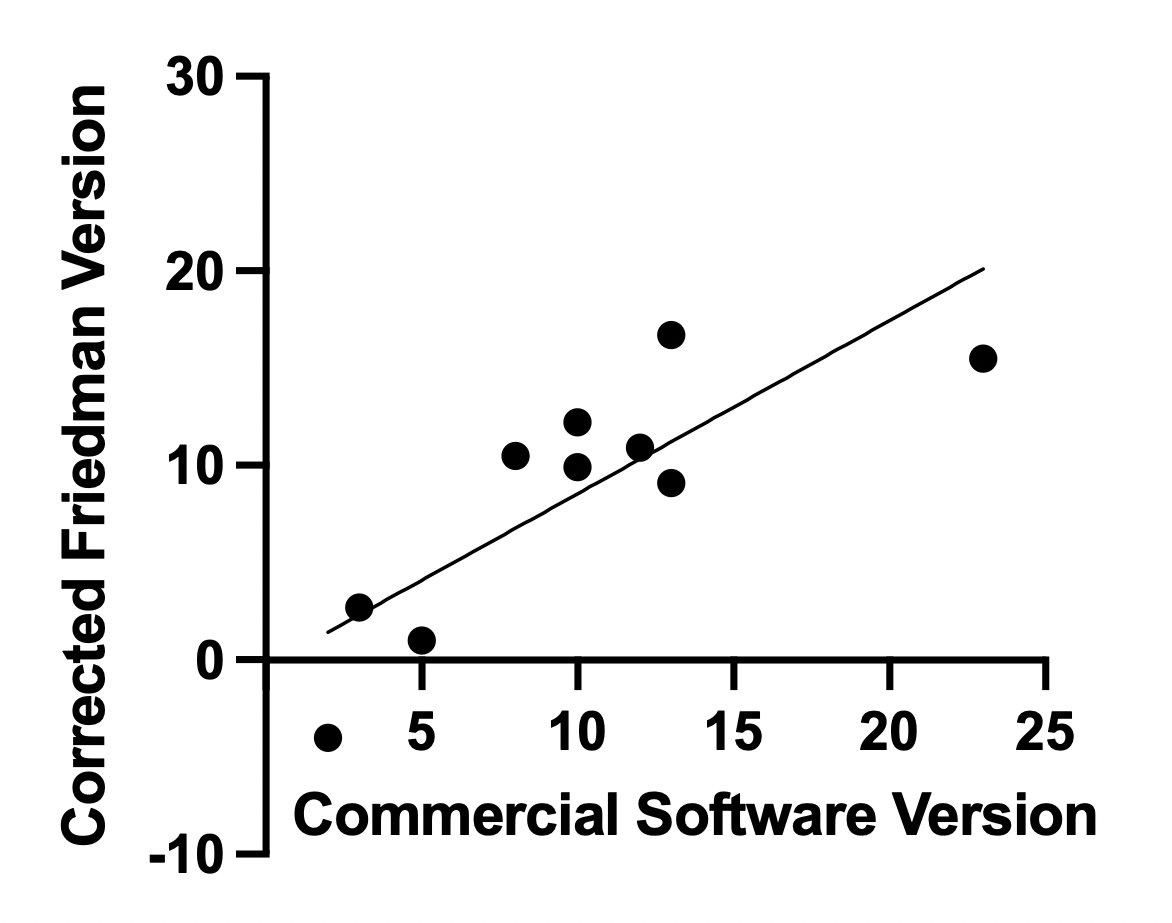
\includegraphics[width=\linewidth]{figures/correctedfried.png}
			\caption{Corrected Friedman Method}
		\end{subfigure}
		\begin{subfigure}[b]{0.30\linewidth}
			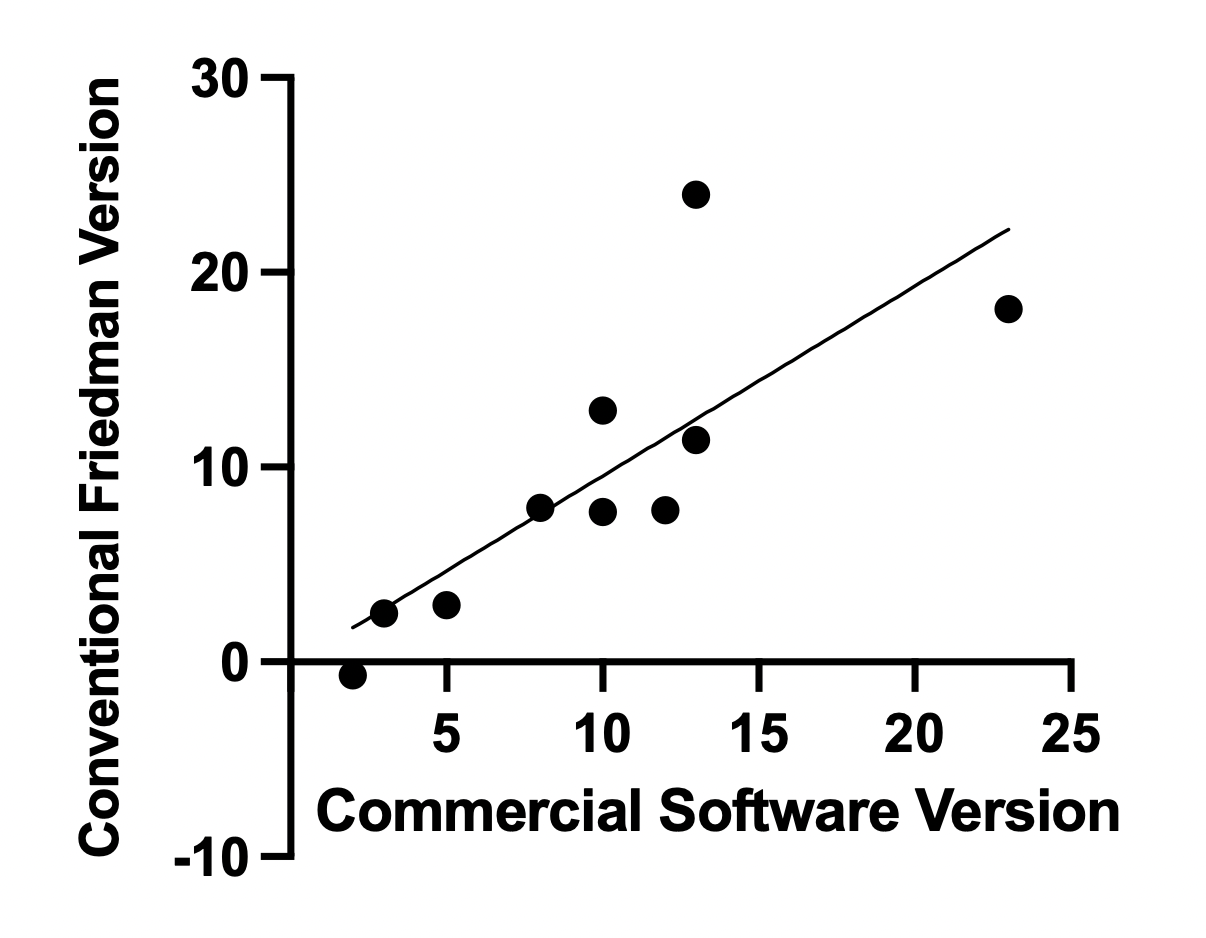
\includegraphics[width=\linewidth]{figures/friedman.png}
			\caption{Friedman Method}
		\end{subfigure}
		\caption{\label{fig:correl}The Pearson correlation between the commercial software and 3 of the methods. All show significant correlation.}
	\end{center}
\end{figure}
